\documentclass[boxes]{homework}

% This is a slightly-more-than-minimal document that uses the homework class.
% See the README at http://git.io/vZWL0 for complete documentation.

\name{傅申 PB20000051}        % Replace (Your Name) with your name.
\term{2022 秋}     % Replace (Current Term) with the current term.
\course{算法基础}    % Replace (Course Name) with the course name.
\hwnum{1}          % Replace (Number) with the number of the homework.
\hwname{作业}
\problemname{}
\solutionname{解:}

% Load any other packages you need here.
\usepackage[
    a4paper,
    top = 2.54cm,
    bottom = 2.54cm,
    left = 1.91cm,
    right = 1.91cm,
    includeheadfoot
]{geometry}
\fancyfootoffset{0pt} % make fancyhdr work properly
\usepackage{ctex}
\usepackage{tikz}
\usetikzlibrary{trees, arrows}

\begin{document}
\problemchap{2}
\problempart{1}

%%%% Problem 2.1-3 %%%%
\problemnumber{3}
\begin{problem}
\label{prob:2.1-3}
考虑以下\textbf{查找问题}:\\
\textbf{输入}: $n$ 个数的一个序列 $A = \left\langle a_1, a_2, \cdots, a_n
    \right\rangle$ 和一个值 $v$.\\
\textbf{输出}: 下标 $i$ 使得 $v = A[i]$ 或者当 $v$ 不在 $A$ 中出现时,
$i$ 为特殊值 NIL.\\
写出\textbf{线性查找}的伪代码, 它扫描整个序列来查找 $v$. 使用一个循环不变式
来证明你的算法是正确的. 确保你的循环不变式满足三条必要的性质.
\end{problem}

\begin{solution}
    线性查找的伪代码如下

    \begin{algo}
        \caption{LINEAR-SEARCH($A$, $v$)}
        \label{algo:linear-search}
        $i = \text{NIL}$\;
        \For{$j = 1$ \textbf{to} $A.length$}{
            \If{$A[j] = v$}{
                $i = j$\;
                \Return $i$\;
            }
        }
        \Return $i$\;
    \end{algo}

    令循环不变式为 ``在开始第 2 \textasciitilde 5 行 \textbf{for} 循环的每次迭
    代时, $v$ 不在子数组 $A[1..j-1]$ 中出现且 $i = \mathrm{NIL}$'', 正确性证明
    如下:
    \begin{description}[
            leftmargin  = !,
            labelindent = 2em,
            labelwidth  = \widthof{\bfseries 初始化},
            topsep      = 0pt,
            itemsep     = 0pt,
            parsep      = 0pt
        ]
        \item[初始化] 在第一次循环迭代之前 (即 $j = 1$ 时), $i = \mathrm{NIL}$,
            子数组 $A[1..j-1]$ 中没有元素, 因此 $v$ 不在子数组 $A[1..j-1]$ 中出
            现, 循环不变式成立.
        \item[保持] 设第 $j$ 次循环迭代之前循环不变式成立. 在第 $j$ 次循环迭代
            中, 如果 $A[j] = v$, 则设置 $i = j$, 循环终止, 不再有下次循环迭代.
            因此若存在下一次循环迭代, 有 $A[j] \neq j$, $i$ 将不会被修改 (保持
            NIL), 并且因为 $v$ 也不在 $A[1..j-1]$ 中出现, $v$ 不在子数组
            $A[1..j]$ 中出现, 循环不变式成立.
        \item[终止] 导致 \textbf{for} 循环终止的条件有两种: 一种情况是 $A[j] =
                v$. 这种情况下会在第 $j$ 次循环迭代中进入第 3 行的 \textbf{if}
            语句, 从而设置 $i = j$ 并返回, 因此得到的下标 $i$ 满足 $v = A[i]$.
            另一种情况是 $j > A.length$, 因为每次循环迭代 $j$ 增加 1, 所以 $j =
                n + 1$. 在循环不变式的表述中将 $j$ 用 $n + 1$ 替换, 得到 $v$ 不
            在子数组 $A[1..n]$ 中出现且 $i = \mathrm{NIL}$. 子数组 $A[1..n]$ 就
            是整个数组, 所以 $v$ 不在整个数组中出现且 $i = \mathrm{NIL}$. 在两
            种情况下都满足要求, 因此算法正确.
    \end{description}
\end{solution}

%%%% Problem 2.1-4 %%%%
\problemnumber{4}
\begin{problem}
考虑把两个 $n$ 位二进制整数加起来的问题, 这两个整数分别存储在两个 $n$ 元数组
$A$ 和 $B$ 中. 这两个整数的和应按二进制形式存储在一个 $(n + 1)$ 元数组 $C$ 中.
请给出该问题的形式化描述, 并写出伪代码.
\end{problem}
\begin{solution}
    形式化描述如下:\\
    \textbf{输入}: 两个 $n$ 元数组 $A = \left\langle a_1, a_2, \cdots, a_n
        \right\rangle, B = \left\langle b_1, b_2, \cdots, b_n\right\rangle$, 其
    中对于所有下标 $i$ 都有 $a_i, b_i \in \{0, 1\}$.\\
    \textbf{输出}: 一个 $(n + 1)$ 元数组 $C = \left\langle c_1, c_2, \cdots,
        c_{n + 1}\right\rangle$, 其中对于所有下标 $i$ 都有 $c_i \in \{0, 1\}$,
    且满足$\displaystyle\sum_{i = 1}^{n + 1} c_i 2^{n + 1 - i} = \sum_{i = 1}^n
        a_i 2^{n - i} + \sum_{i = 1}^n b_i 2^{n - i}$.

    算法伪代码如下:

    \begin{algo}
        \caption{BINARY-ADD ($A, B$)}
        \label{alg:binary-add}

        $carry = 0$\;
        \For{$i = n$ \textbf{downto} 1}{
            $C[i + 1] = A[i] + B[i] + carry$\;
            \eIf{$C[i + 1] \geqslant 2$}{
                $C[i + 1] = C[i + 1] - 2$\;
                $carry = 1$\;
            } {
                $carry = 0$\;
            }
        }
        $C[1] = carry$\;
    \end{algo}
\end{solution}

%%%% Problem 2.2-2 %%%%
\problempart{2}
\problemnumber{2}
\begin{problem}
考虑排序存储在数组 $A$ 中的 $n$ 个数: 首先找出 $A$ 中最小元素并将其与 $A[1]$ 中
的元素进行交换. 接着, 找出 $A$ 中的次最小元素并将其与 $A[2]$ 中的元素进行交换.
对 $A$ 中前 $n - 1$ 个元素按该方式继续. 该算法称为\textbf{选择算法}, 写出其伪代
码. 该算法维持的循环不变式是什么? 为什么它只需要对前 $n - 1$, 而不是对所有 $n$
个元素进行? 用 $\Theta$ 记号给出选择排序的最好情况与最坏运行情况运行时间.
\end{problem}

\begin{solution}
    选择算法的伪代码如下:

    \begin{algo}
        \caption{SELECTION-SORT ($A$)}
        \label{alg:selection-sort}
        \For{$j = 1$ \textbf{to} $A.length - 1$}{
            $min = j$\;
            \For{$i = j + 1$ \textbf{to} $A.length$}{
                \If{$A[i] < A[min]$}{
                    $min = i$\;
                }
            }
            $temp = A[j]$\;
            $A[j] = A[min]$\;
            $A[min] = temp$\;
        }
    \end{algo}

    该算法维持的循环不变式为 ``在第 1 \textasciitilde 8 行的 \textbf{for} 循环
    的每次迭代开始时, 子数组 $A[1 .. j - 1]$ 由原数组 $A[1 .. n]$ 中前 $j - 1$
    小元素组成, 且已按序排列, $A[j .. n]$ 由原数组 $A[1 .. n]$ 中后 $n - j + 1$
    小元素组成''.

    该算法只需要对前 $n - 1$ 个元素进行, 因为在第 $n - 1$ 次迭代后, 子数组 $A[1
                .. n - 1]$ 由原数组 $A[1 .. n]$ 中前 $n - 1$ 小元素组成, 且已按序排列, 而
    此时 $A[n]$ 中就是原数组中最大的元素, 整个数组已按序排列.

    假设第 $i$ 行的运行时间为 $c_{i}$. 当输入数组按升序排列时, 出现最佳情况, 运
    行时间为
    \begin{equation}
        \label{eq:1}
        \begin{aligned}
            T_{\min}(n) & = \sum_{j = 1}^{n - 1} \left( c_{1} + c_{2} +
            \sum_{i = j + 1}^{n} \left( c_{3} + c_{4}\right) + c_{6} + c_{7} +
            c_{8} \right)                                                     \\
                        & = \frac{c_{3} + c_{4}}{2} \, n^{2} + \left( c_{1} +
            c_{2} + c_{6} + c_{7} + c_{8} - \frac{c_{3} + c_{4}}{2}\right) n  \\
                        & = \Theta(n^{2})
        \end{aligned}
    \end{equation}
    当输入数组按降序排列时, 出现最坏情况, 运行时间为
    \begin{equation}
        \label{eq:2}
        \begin{aligned}
            T_{\max}(n) & = \sum_{j = 1}^{n - 1} \left( c_{1} + c_{2} +
            \sum_{i = j + 1}^{n} \left( c_{3} + c_{4} + c_{5}\right) + c_{6} +
            c_{7} + c_{8}\right)                                           \\
                        & = \frac{ c_{3} + c_{4} + c_{5} }{ 2 } \, n^{2} +
            \left( c_{1} + c_{2} + c_{6} + c_{7} + c_{8} - \frac{ c_{3} + c_{4}
            + c_{5} }{ 2 }\right) n                                        \\
                        & = \Theta(n^{2})
        \end{aligned}
    \end{equation}
\end{solution}

%%%% Problem 2.2-3 %%%%
\begin{problem}
再次考虑线性查找问题 (参见练习 \hyperref[prob:2.1-3]{2.1--3}). 假定要查找的元素
等可能的为数组中的任意元素, 平均需要检查输入序列的多少元素? 最坏情况又如何呢?
用 $\Theta$ 记号给出线性查找的平均情况和最坏情况运行时间. 证明你的答案.
\end{problem}
\begin{solution}
    数组中每个元素被查找的概率均为 $\dfrac{ 1 }{ n }$, 所以平均需要检查输入序列
    的 $\displaystyle \sum_{j = 1}^{n} \frac{ j }{ n } = \frac{ n + 1 }{ 2 }$
    个元素. 在平均情况下, 运行时间
    \begin{equation}
        \label{eq:3}
        \begin{aligned}
            T_{\mathrm{avg}}(n) & = c_{1} + \frac{ n + 1 }{ 2 } \left( c_{2} +
            c_{3}\right) + c_{4} + c_{5}                                       \\
                                & = \frac{ c_{2} + c_{3} }{ 2 } n + c_{1} +
            c_{4} + c_{5} + \frac{ c_{2} + c_{3} }{ 2 }                        \\
                                & = \Theta(n)
        \end{aligned}
    \end{equation}

    当数组中没有需要查找的元素或者需要查找的元素为数组中最后一个元素时, 出现最坏
    情况, 需要检查输入序列的所有元素, 也就是 $n$ 个元素. 在最坏情况下 (假设没有
    找到需要的元素), 运行时间为
    \begin{equation}
        \label{eq:4}
        T_{\max}(n) = \left( c_{2} + c_{3} \right)n + c_{1} + c_{6} = \Theta(n)
    \end{equation}
\end{solution}

%%%% Problem 2.3-1 %%%%
\problempart{3}
\problemnumber{1}
\begin{problem}
使用书上图 2--4 作为模型, 说明归并排序在数组 $A = \left\langle 3, 41, 52, 26,
    38, 57, 9, 49\right\rangle$ 上的操作.
\end{problem}
\begin{solution}
    操作如下:

    \begin{figure}[!htbp]
        \centering
        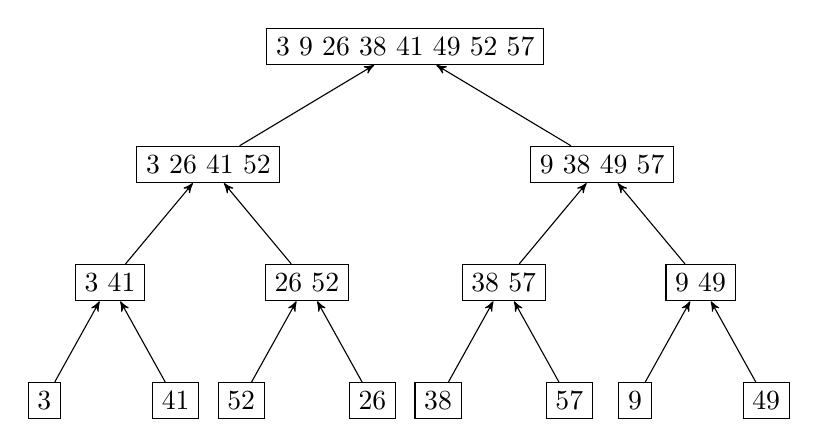
\begin{tikzpicture}[<-, >=stealth',
                every node/.style={rectangle, draw, fill=none},
                level/.style={sibling distance=5cm/#1, level distance=1.5cm}]
            \node{3 9 26 38 41 49 52 57}
            child{node{3 26 41 52}
                    child{node{3 41}
                            child{node{3}}
                            child{node{41}}
                        }
                    child{node{26 52}
                            child{node{52}}
                            child{node{26}}
                        }
                }
            child{node{9 38 49 57}
                    child{node{38 57}
                            child{node{38}}
                            child{node{57}}
                        }
                    child{node{9 49}
                            child{node{9}}
                            child{node{49}}
                        }
                };
        \end{tikzpicture}
        \caption{归并排序的操作}
        \label{fig:merge-sort}
    \end{figure}
\end{solution}

%%%% Problem 2.3-5 %%%%
\problemnumber{5}
\begin{problem}
回顾查找问题 (参见练习 \hyperref[prob:2.1-3]{2.1--3}). 注意到, 如果序列 $A$ 已
排好序, 就可以将该序列的中点与 $v$ 进行比较. 根据比较的结果, 原序列有一半就可以
不用再做进一步的考虑了. \textbf{二分查找} 算法重复这个过程, 每次都将序列剩余部分
的规模减半. 为二分查找写出迭代或递归的伪代码, 证明: 二分查找的最坏情况运行时间
为 $\Theta(\lg n)$.
\end{problem}
\begin{solution}
    二分查找的伪代码如下, 其中初始调用为 BINARY-SEARCH($A$, $v$, $1$, $n$):
    \begin{algo}
        \caption{BINARY-SEARCH($A$, $v$, $p$, $r$)}
        \label{algo:binary-search}

        \If{$p > r$}{
            \Return NIL\;
        }
        $q = \left\lfloor \dfrac{ p + r }{ 2 } \right\rfloor$\;
        \uIf{$v = A[q]$}{
            \Return $q$\;
        }
        \uElseIf{$v > A[q]$}{
            \Return BINARY-SEARCH($A$, $v$, $q + 1$, $r$)\;
        }
        \Else{
            \Return BINARY-SEARCH($A$, $v$, $p$, $q - 1$)\;
        }
    \end{algo}
    分解过程只需要检查下标并计算中间下标, 需要常量时间, $D(n) = \Theta(1)$; 在
    最坏情况下, 解决过程每次都需要递归地求解一个规模为 $\dfrac{ n }{ 2 }$ 的子
    问题, 贡献 $T \left( \dfrac{ n }{ 2 }\right)$ 的运行时间, 直到子数组长度小
    于等于 1; 合并过程只需要返回下标, 需要常量时间, $C(n) = \Theta(1)$. 因此,
    最坏情况运行时间的递推式为
    \begin{equation}
        \label{eq:5}
        T(n) =
        \begin{cases}
            \Theta(1)                                    & n \leq 1 \\
            T \left( \dfrac{ n }{ 2 }\right) + \Theta(1) & n > 1
        \end{cases}
    \end{equation}
    运用递归树, 每一层都只有一个结点, 代价均为 $\Theta (1)$, 高度至多为
    $\lceil\lg n + 1\rceil$, 因此 $T(n)$ 为 $\Theta(\lg n)$.
\end{solution}

%%%% Problem 3.1-2 %%%%
\problemchap{3}
\problempart{1}
\problemnumber{2}
\begin{problem}
证明: 对任意实常量 $a$ 和 $b$, 其中 $b > 0$, 有
\begin{equation}
    {(n + a)}^{b} = \Theta \left( n^{b}\right)
\end{equation}
\end{problem}
\begin{solution}
    取 $c_{1} = {\left( \dfrac{ 1 }{ 2 }\right)}^{b}$, $c_{2} = {\left(
                \dfrac{ 3 }{ 2 }\right)}^{b}$ 和 $n_{0} = 2 \left\lvert a
        \right\rvert$, 当 $n \geqslant n_{0}$ 时, 有
    \begin{equation}
        \frac{ 3 }{ 2 } n \geqslant n + \left\lvert a\right\rvert \geqslant
        n + a \geqslant n - \left\lvert a\right\rvert \geqslant
        \frac{ 1 }{ 2 }n \geqslant 0
    \end{equation}
    因此就有
    \begin{equation}
        c_{2} n^{b} = {\left( \frac{ 3 }{ 2 }n\right)}^{b} \geqslant
        {\left( n + a\right)}^{b} \geqslant {\left( \frac{1}{2} n\right)}^{b}
        = c_{1} n^{b} \geqslant 0
    \end{equation}
    所以 ${(n + a)}^{b} = \Theta \left( n^{b}\right)$
\end{solution}

%%%% Problem 3.1-4 %%%%
\problemnumber{4}
\begin{problem}
$2^{n + 1} = O \left( 2^{n}\right)$ 成立吗? $2^{2n} = O \left( 2^{n}\right)$
成立吗?
\end{problem}
\begin{solution}
    $2^{n + 1} = O\left( 2^{n}\right)$ 成立. 取 $c = 3$ 和 $n_{0} = 1$, 当 $n
        \geqslant n_{0}$ 时, 有
    \begin{equation}
        0 \leqslant 2^{n + 1} \leqslant 3 \times 2^{n} = c \times 2^{n}
    \end{equation}

    $2^{2n} = O \left( 2^{n}\right)$ 不成立. 对任意的实常量 $c$, 当 $n > \lg c$
    时, 有
    \begin{equation}
        2^{2n} = 2^{n} \cdot 2^{n} \geqslant c \times 2^{n}
    \end{equation}
\end{solution}

%%%% 3.1-6 %%%%
\problemnumber{6}
\begin{problem}
证明: 一个算法的运行时间为 $\Theta \left( g(n)\right)$ 当且仅当其最坏情况运行时
间为 $O \left( g(n)\right)$ 且其最好情况运行时间为 $\Omega \left( g(n)\right)$.
\end{problem}
\begin{solution}
    记算法的运行时间, 最坏情况运行时间和最好情况运行时间分别为 $T(n)$, $T_{\max
            }(n)$ 和 $T_{\min}(n)$, 则有
    \begin{equation}
        T_{\min}(n) \leqslant T(n) \leqslant T_{\max}(n)
    \end{equation}

    先证明 $T_{\max}(n) = O(g(n)), T_{\min}(n) = \Omega(g(n))
        \Rightarrow T(n) = \Theta(g(n))$.
    因为 $T_{\min}(n) = \Omega \left( g(n)\right)$, 所以存在正常量 $c_{1}$ 和
    $n_{1}$, 当 $n \geqslant n_{1}$ 时, 有
    \begin{equation}
        c_{1} g(n) \leqslant T_{\min}(n)
    \end{equation}
    同理, $T_{\max}(n) = O \left( g(n)\right)$, 所以存在正常量 $c_{2}$ 和
    $n_{2}$, 当 $n \geqslant n_{2}$ 时, 有
    \begin{equation}
        T_{\max}(n) \leqslant c_{2} g(n)
    \end{equation}
    因此, 取 $n_{0} = \max \left\{ n_{1}, n_{2}\right\}$, 当 $n \geqslant
        n_{0}$ 时, 有
    \begin{equation}
        c_{1} g(n) \leqslant T_{\min}(n) \leqslant T(n) \leqslant T_{\max}(n)
        \leqslant c_{2} g(n)
    \end{equation}
    所以 $T(n) = \Theta \left( g(n)\right)$.

    再证明 $T(n) = \Theta(g(n)) \Rightarrow T_{\max}(n) = O(g(n)),
        T_{\min}(n) = \Omega(g(n))$.
    因为 $T(n) = \Theta \left( g(n)\right)$, 所以存在正常量 $c_{1}$, $c_{2}$ 和
    $n_{0}$, 当 $n \geqslant n_{0}$ 时, 在所有情况下有
    \begin{equation}
        c_{1} g(n) \leqslant T_{\min} \leqslant T(n) \leqslant T_{\max}(n)
        \leqslant c_{2} g(n)
    \end{equation}
    所以显然有 $T_{\max}(n) = O(g(n))$, $T_{\min}(n) = \Omega(g(n))$.
\end{solution}

%%%% Problem 3.2-3 %%%%
\problempart{2}
\problemnumber{3}
\begin{problem}
证明下面的等式. 并证明 $n! = \omega \left( 2^{n}\right)$ 且 $n! = o \left(
    n^{n}\right)$.
\begin{equation}
    \lg \left( n!\right) = \Theta \left( n\lg n\right)
\end{equation}
\end{problem}
\begin{solution}
    首先证明 $\lg \left( n!\right) = \Theta \left( n \lg n\right)$. 取 $c_{1} =
        \dfrac{ 1 }{ 2 }$, $c_{2} = 1$, 和 $n_{0} = \mathrm{e}^{2}$, 当 $n
        \geqslant n_{0}$ 时, 有
    \begin{gather}
        \label{eq:7}
        \lg \left( n!\right) = \lg \left( \sqrt{2\pi n} {\left( \frac{ n }{
                \mathrm{e} }\right)}^{n} \mathrm{e}^{\alpha_{n}}\right) =
        \frac{ 1 }{ 2 }\lg \left( 2\pi\right) + \frac{ 1 }{ 2 }\lg n +
        n\lg \left( \frac{ n }{ \mathrm{e} }\right) + \alpha_{n}\lg
        \mathrm{e} \geqslant n\lg \left( \frac{ n }{ \mathrm{e} }\right)
        \geqslant n\lg \left( \sqrt{n}\right) = \frac{ 1 }{ 2 } n\lg n\\
        \lg \left( n!\right) = \sum_{i = 1}^{n} \lg i \leqslant
        \sum_{i = 1}^{n} \lg n = n\lg n = c_{2} n\lg n
    \end{gather}

    然后证明 $n! = \omega \left( 2^{n}\right)$. 对任意正常量 $c > 0$, 取 $n_{0}
        = \max\{5, 2c + 1\}$, 当 $n \geqslant n_{0}$ 时, 有
    \begin{equation}
        n! =
        \begin{cases}
            \dfrac{ n! }{ 5! } \times 5! > 2^{n - 5} \times 120 > c \times
            2^{n}                                               & 0 < c \leqslant 2 \\
            \dfrac{ n! }{ 1! } \geqslant 2^{2} \times \left\lfloor
            \dfrac{ n }{ 2 } \right\rfloor \times \left\lfloor \dfrac{ n - 1 }
            { 2 } \right\rfloor \times \dfrac{ (n - 2)! }{ 1! } \geqslant 2^{2}
            \times c \times 2 \times 2^{n - 3} = c \times 2^{n} & c > 2
        \end{cases}
    \end{equation}

    最后证明 $n! = o \left( n^{n}\right)$. 对任意正常量 $c > 0$, 取 $n_{0} =
        \max \left\{ \dfrac{ 1 }{ c }, 1 \right\}$, 当 $n \geqslant n_{0}$ 时,
    有
    \begin{equation}
        n!
        \begin{cases}
            = \dfrac{ n! }{ 1! } \leqslant n^{n - 1} \leqslant n^{n - 1} \times
            cn                       & 0 < c \leqslant 1 \\
            \leqslant n^{n} < cn^{n} & c > 1
        \end{cases}
    \end{equation}
\end{solution}

%%%% Problem 3.2-5 %%%%
\problemnumber{5}
\begin{problem}
如下两个函数中, 哪个渐进更大些: $\lg \left( \lg^{*} n\right)$ 还是 $\lg^{*}
    \left( \lg n\right)$?
\end{problem}
\begin{solution}
    记 $n = 2^{m}$, $t = \lg^{*} m$, 就有
    \begin{gather}
        \lg \left( \lg^{*} n\right) = \lg \left( 1 + \lg^{*} m\right) = \lg
        \left( 1 + t\right) \\
        \lg^{*} \left( \lg n\right) = \lg^{*} m = t
    \end{gather}
    因此, 原题转化为比较 $\lg \left( 1 + t\right)$ 和 $t$ 的渐进大小, 有 $\lg
        \left( 1 + t\right) = o \left( t\right)$, 证明如下.

    首先证明当 $x > 1$ 时有 $\ln x < 2 \sqrt{x} - 2$, 因为当 $x > 1$ 时有 $\ln
        x < x - 1$, 所以
    \begin{equation}
        \ln \sqrt{x} = \frac{ 1 }{ 2 } \ln x < \sqrt{x} - 1 \iff \ln x <
        2\sqrt{x} - 2
    \end{equation}

    对任意正常量 $c > 0$, 记 $b = c\ln 2$, 取 $t_{0} = \max \left\{
        \dfrac{ 4 - 4b }{ b^{2} }, 1\right\}$, 当 $t \geqslant t_{0}$ 时, 有
    \begin{equation}
        \begin{aligned}
            \lg \left( 1 + t\right) \leqslant ct
             & \impliedby \ln \left( 1 + t \right) \leqslant ct\ln 2 = bt     \\
             & \impliedby 2\sqrt{1 + t} - 2 \leqslant bt                      \\
             & \impliedby b^{2}t^{2} + \left( 4b - 4\right)t \geqslant 0      \\
             & \impliedby t \geqslant \frac{ 4 - 4b }{ b^{2} } \text{ 且 }\ t
            \geqslant 1
        \end{aligned}
    \end{equation}

    综上所述, 有 $\lg \left( \lg^{*} n\right) = o\left( \lg^{*} \left( \lg n
            \right)\right)$, 即 $\lg^{*} \left( \lg n\right)$ 的渐进更大.
\end{solution}
\end{document}
